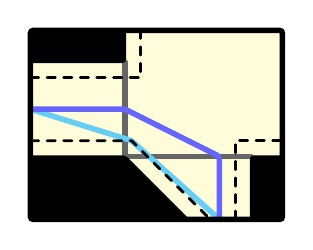
\begin{tikzpicture}[thick,scale=0.4, every node/.style={scale=0.4}]

\tikzset{cross/.style={thick, cross out, line width=4, minimum size=10pt, inner sep=0pt, outer sep=0pt},
%default radius will be 1pt. 
cross/.default={1pt}}

\begin{scope}

\clip (0,0) -- (8,0) -- (8,6) -- (0,6) -- cycle;

\draw [line width=0,fill=yellow!15!white] (0,0) -- (8,0) -- (8,6) -- (0,6) -- cycle;

\draw [black!60!white,line width=2,line cap=round] (3,2) -- (3,5);
\draw [black!60!white,line width=2,line cap=round] (3,2) -- (7,2);

\draw [fill=black,rounded corners=1] (0,0) -- (0,2) -- (3,2) -- (5,0) -- cycle;
\draw [fill=black,rounded corners=1] (0,5) -- (0,6) -- (3,6) -- (3,5) -- cycle;
\draw [fill=black,rounded corners=1] (7,0) -- (7,2) -- (8,2) -- (8,0) -- cycle;

\draw [cyan!60!white,line width=2,line cap=round,rounded corners=1] (0,3.5) -- (3.21,2.5) -- (6,0);
\draw [blue!60!white,line width=2,line cap=round,rounded corners=1] (0,3.5) -- (3,3.5) -- (6,2) -- (6,0);

\draw [black,line width=1,line cap=round,dashed] (0,2.5) -- (3.21,2.5) -- (5.71,0);
\draw [black,line width=1,line cap=round,dashed] (6.5,0) -- (6.5,2.5) -- (8,2.5);
\draw [black,line width=1,line cap=round,dashed] (0,4.5) -- (3.5,4.5) -- (3.5,6);

\end{scope}

\draw [line width=2,rounded corners=1] (0,0) -- (8,0) -- (8,6) -- (0,6) -- cycle;

\end{tikzpicture}